\documentclass{beamer}
\usetheme{Madrid}
\usecolortheme{spruce}

\usepackage{graphicx}
\usepackage{csquotes}
\usepackage{tabularx}
\usepackage{pifont}
\usepackage[czech]{babel}
\usepackage[style=iso-numeric]{biblatex}
\addbibresource{refs.bib}

\title[Hodnocení kryptografických knihoven]{Kritéria pro hodnocení bezpečnosti\\kryptografických knihoven}
\subtitle{Bakalářská práce}
\author[Milan Špinka]{\texorpdfstring{Milan Špinka\\[0.5em]pod vedením Ing.\,Josefa~Kokeše,\,Ph.D.}{Milan Špinka}}
\date{20.\ června 2024}

\newcommand{\textbc}[1]{{\usebeamercolor[fg]{titlelike} #1}}

\newenvironment{spaceditemize}[1][1em]
{ \begin{itemize}
    \setlength{\itemsep}{#1}
%    \setlength{\parskip}{0pt}
%    \setlength{\parsep}{0pt}
%    \vspace{#1}
}{ \end{itemize} } 

\begin{document}
\setbeamertemplate{page number in head/foot}{}
\maketitle
\setbeamertemplate{page number in head/foot}[appendixframenumber]

%--------------------%
\section{Předmět práce}
%--------------------%

\begin{frame}{Motivace a cíle práce I}
    Vývojáři aplikací potřebují použít kryptografii --- jak?
    \begin{figure}
        \centering
        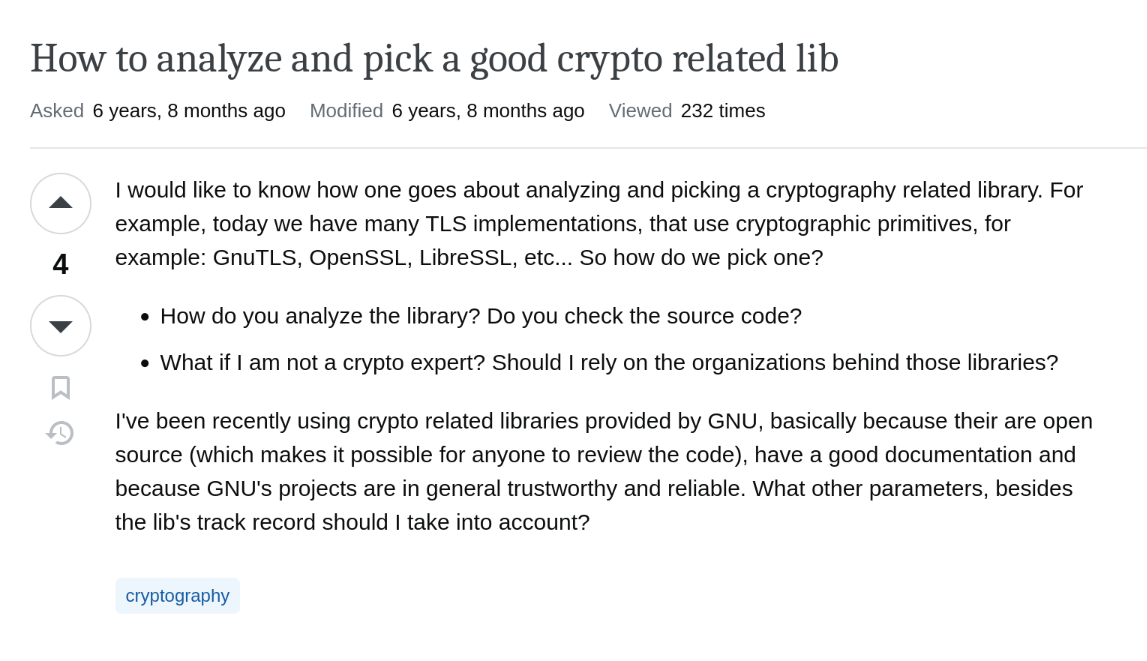
\includegraphics[width=0.8\textwidth]{media/stackexchange.png}
        \caption{Příklad dotazu na fóru Stack Exchange \cite{stackexchange} směřující na metody hodnocení/porovnání kryptografických knihoven.}
        \label{fig:stackexchange}
    \end{figure}
\end{frame}

\begin{frame}{Motivace a cíle práce II}
    \textbf{\textbc{Zadání}}
    \vspace{.5em}
    
    \begin{spaceditemize}[0.5em]
        \item Výzkumný projekt Národního úřadu pro kybernetickou a informační bezpečnost \cite{nukib} --- již proběhlo úspěšné oponentní řízení
        \item Řešitelský tým FIT ČVUT --- další výsledky v bakalářských pracích Matěje Douši \cite{matej} a Kirilla Leonova \cite{kirill}
    \end{spaceditemize}

    \vspace{.5em}
    \textbf{\textbc{Výzkumné otázky}}
    \vspace{.5em}

    \begin{spaceditemize}[0.5em]
        \item Jak posoudit důvěryhodnost knihovny?
        \begin{itemize}
            \item Nekompetence vývojářů
            \item Zlomyslní správci (zadní vrátka)
        \end{itemize}

        \item Jak hodnotit bezpečnost její implementace?

        \item Lze zaručit i bezpečné použití knihovny?
    \end{spaceditemize}
\end{frame}

%--------------------%
\section{Metoda}
%--------------------%

\begin{frame}{Strategie --- dílčí cíle}
    \begin{spaceditemize}
        \item Literární rešerše
        \begin{itemize}
            \item Bezpečnost open-source softwaru (OSS)
            \item Bezpečný návrh kryptografických knihoven
            \item Chybné použití kryptografie v praxi
        \end{itemize} 
        
        \item Výběr a analýza 6 kryptografických knihoven
        \begin{itemize}
            \item OpenSSL, libgcrypt (C)
            \item rustls, ring (Rust)
            \item cryptography, PyCryptodome (Python)
        \end{itemize}

        \item Stanovení metody pro hledání častých chyb v použití knihoven
        
        \item Formulace kritérií (heuristik) pro snadné zhodnocení bezpečnosti libovolné kryptografické knihovny
    \end{spaceditemize}
\end{frame}

%--------------------%
\section{Výsledky}
%--------------------%

\begin{frame}{Výsledky}
    Pro bezpečnost je relevantních především 5~aspektů knihoven:
    \vspace{1em}
    \begin{spaceditemize}
        \item Organizace a vývoj
        \item Kvalita kódu
        \item Rozhraní knihovny (API)
        \item Dokumentace
        \item Alternativní zdroje informací
    \end{spaceditemize}
\end{frame}

\begin{frame}{Organizace, vývoj, kvalita kódu}
    \vspace{1em}
    \begin{spaceditemize}
        \item Aktivita vývoje, přispívání, proces revize kódu
        \begin{itemize}
            \item Paradoxně více recenzentů $\rightarrow$ více zranitelností \cite{linuslaw2014}
        \end{itemize}
        \item Motivace správců (obchodní nebo nezisková společnost, open-source komunita, jednotlivec,~\dots)
        \item Testování, reakce na objevené zranitelnosti
        \item \textit{Code review} celé knihovny nepřipadá v úvahu
        \item Alternativní řešení: odhad na základě praktik ve vývoji
        \begin{itemize}
            \item Pokyny pro formátování kódu
            \item Paměťově bezpečné jazyky
            \item Statická analýza
            \item Testování a fuzzing
        \end{itemize}
    \end{spaceditemize}
\end{frame}

\begin{frame}{Rozhraní knihovny}
    \begin{spaceditemize}[1.25em]
        \item Většina zranitelností vznikne \textbc{chybným použitím kryptografie} \cite{iv0security}
        \item Klíčová literatura: Green \& Smith (2017)~\cite{greensmith} --- 10~principů pro návrh~bezpečných kryptografických API
        \item Dále mě zajímalo porovnání programovacích jazyků s různými úrovněmi abstrakce
        \item Aspekty vyhodnocené jako klíčové:
        \begin{itemize}
            \item Vysoká úroveň abstrakce
            \item Kvalitní mechanismus ošetření chyb
            \item Dostatečná flexibilita API
            \item Bezpečné výchozí hodnoty
            \item Silné typování parametrů
        \end{itemize}
    \end{spaceditemize}
\end{frame}

\begin{frame}{Dokumentace I}
    \begin{figure}
        \centering
        \begin{minipage}{0.42\textwidth}
            \centering
            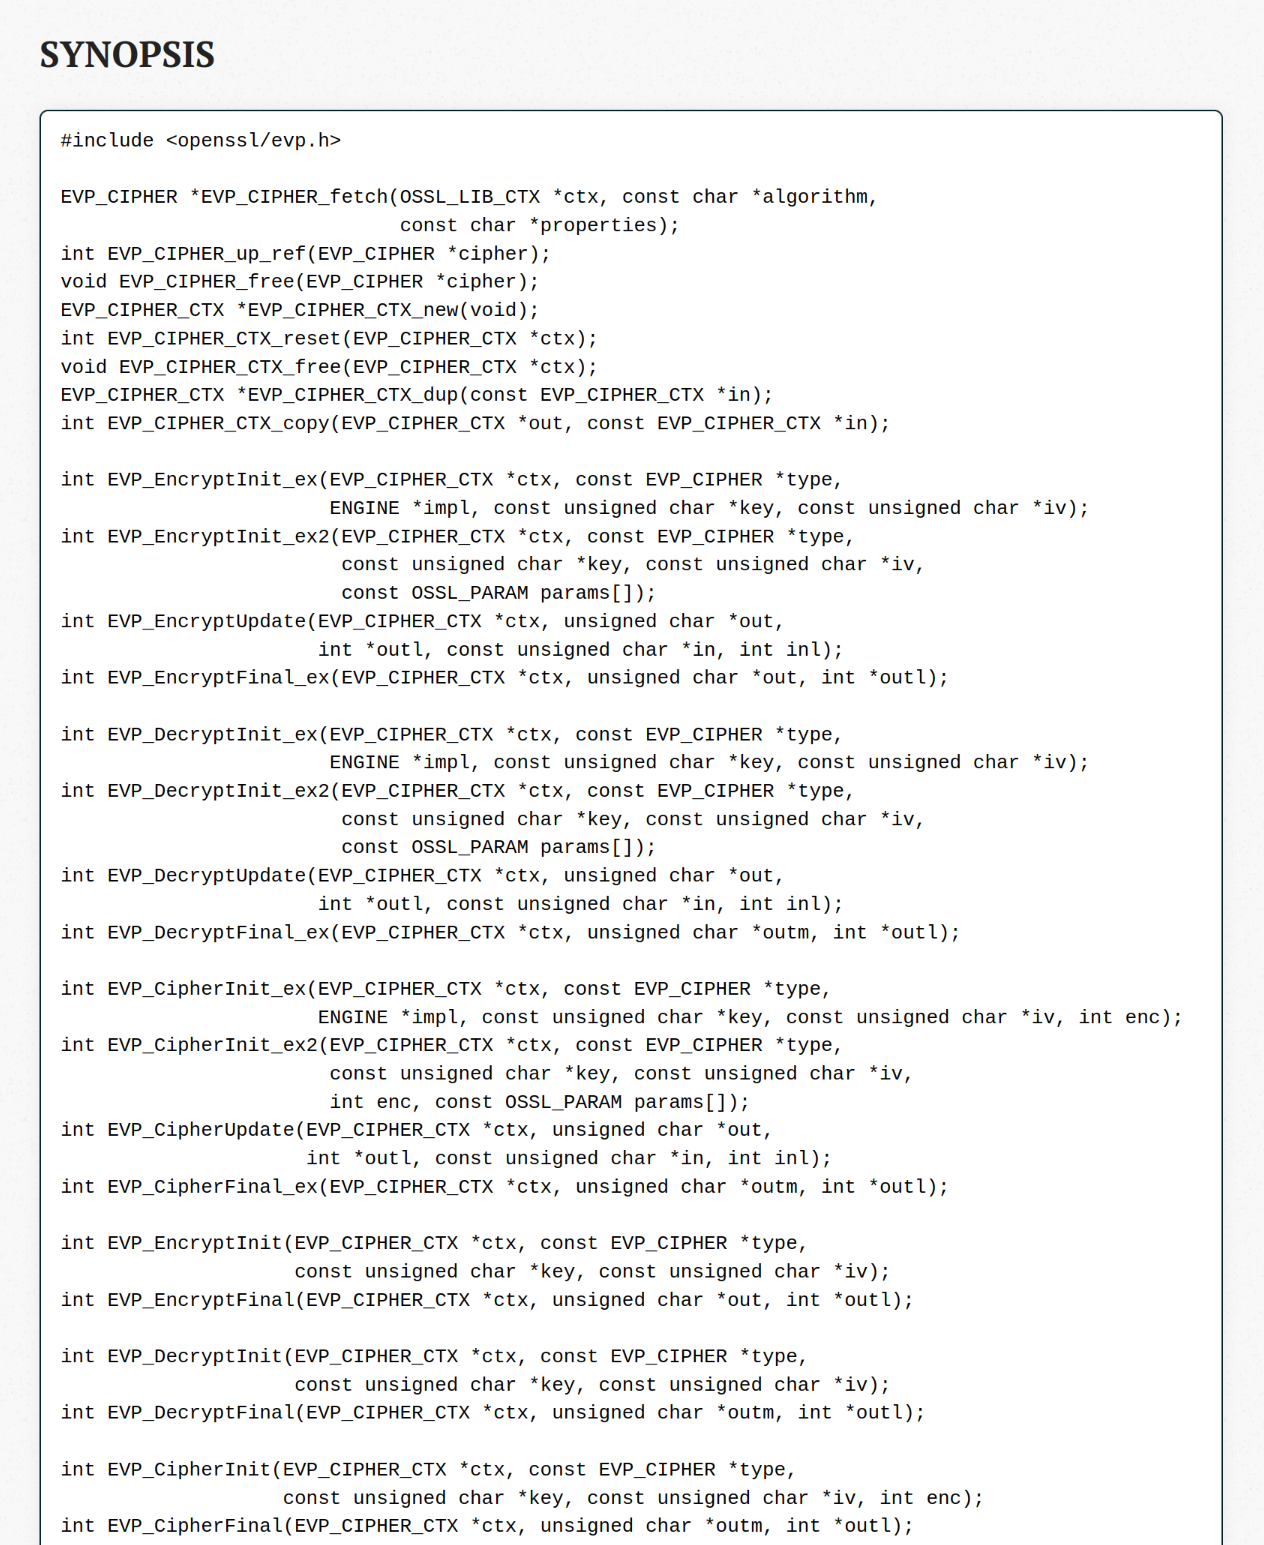
\includegraphics[width=\textwidth]{media/doc-openssl.png}
            \caption{Snímek dokumentace knihovny \textit{OpenSSL} \cite{openssldoc}}
        \end{minipage}\hfill
        \begin{minipage}{0.53\textwidth}
            \centering
            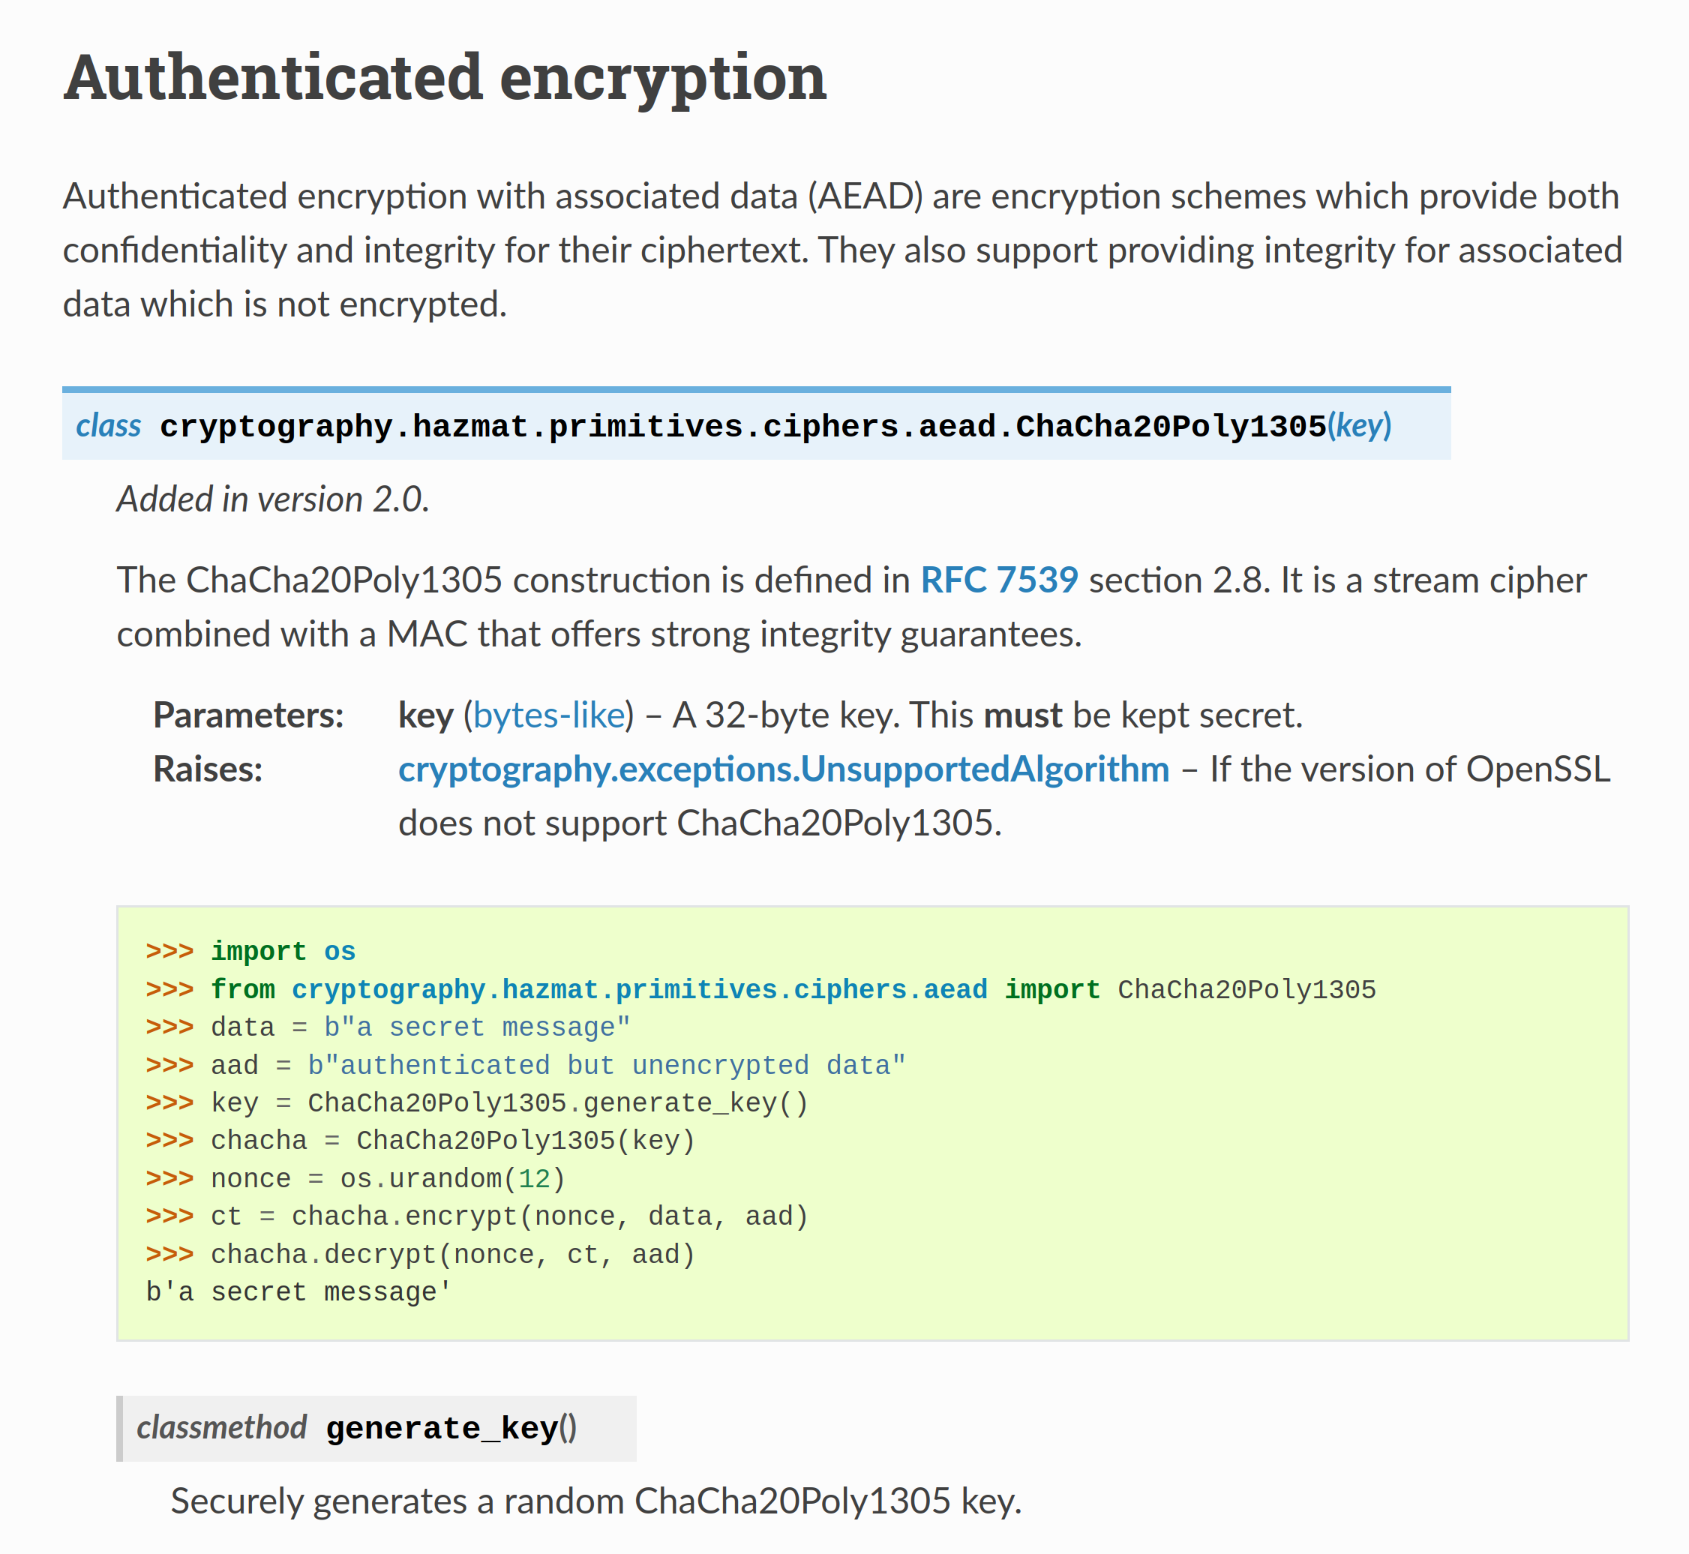
\includegraphics[width=\textwidth]{media/doc-pyca.png}
            \caption{Snímek dokumentace knihovny \textit{cryptography} \cite{pycadoc}}
        \end{minipage}
    \end{figure}
\end{frame}

\begin{frame}{Dokumentace II}
    Klíčové aspekty:
    \vspace{0.5em}
    \begin{spaceditemize}[0.5em]
        \item Úplnost, přehlednost, správnost
        \item Bezpečné a realistické ukázky použití
        \item Vysvětlení algoritmů a parametrů
        \item Oddělení a varování před nebezpečnými konfiguracemi
    \end{spaceditemize}

    \begin{figure}
        \centering
        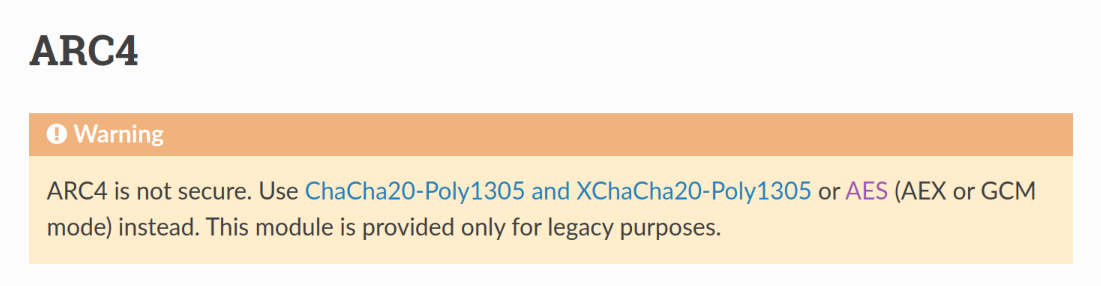
\includegraphics[width=0.8\textwidth]{media/doc-pcd.png}
        \caption{Varování před zastaralou šifrou RC4 v~dokumentaci PyCryptodome \cite{pcddoc}}
    \end{figure}
\end{frame}

\begin{frame}{Zdroje informací I}
    \textbc{Co když dokumentace nezodpoví dotazy uživatele?}

    \vspace{1em}
    Programátoři často používají alternativní zdroje informací \cite{worrisome}:
    
    \vspace{1em}
    \begin{spaceditemize}
        \item Online diskuze (GitHub issues, Stack Overflow)
        \item Online tutoriály
        \item Z těchto zdrojů můžeme odhadnout časté chyby
    \end{spaceditemize}

    \vspace{2em}
    \enskip $\rightarrow$ Jak zanalyzovat obrovské množství neoficiálních zdrojů informací o použití knihovny na internetu?
\end{frame}

\begin{frame}{Zdroje informací II}
    \begin{figure}
        \centering
        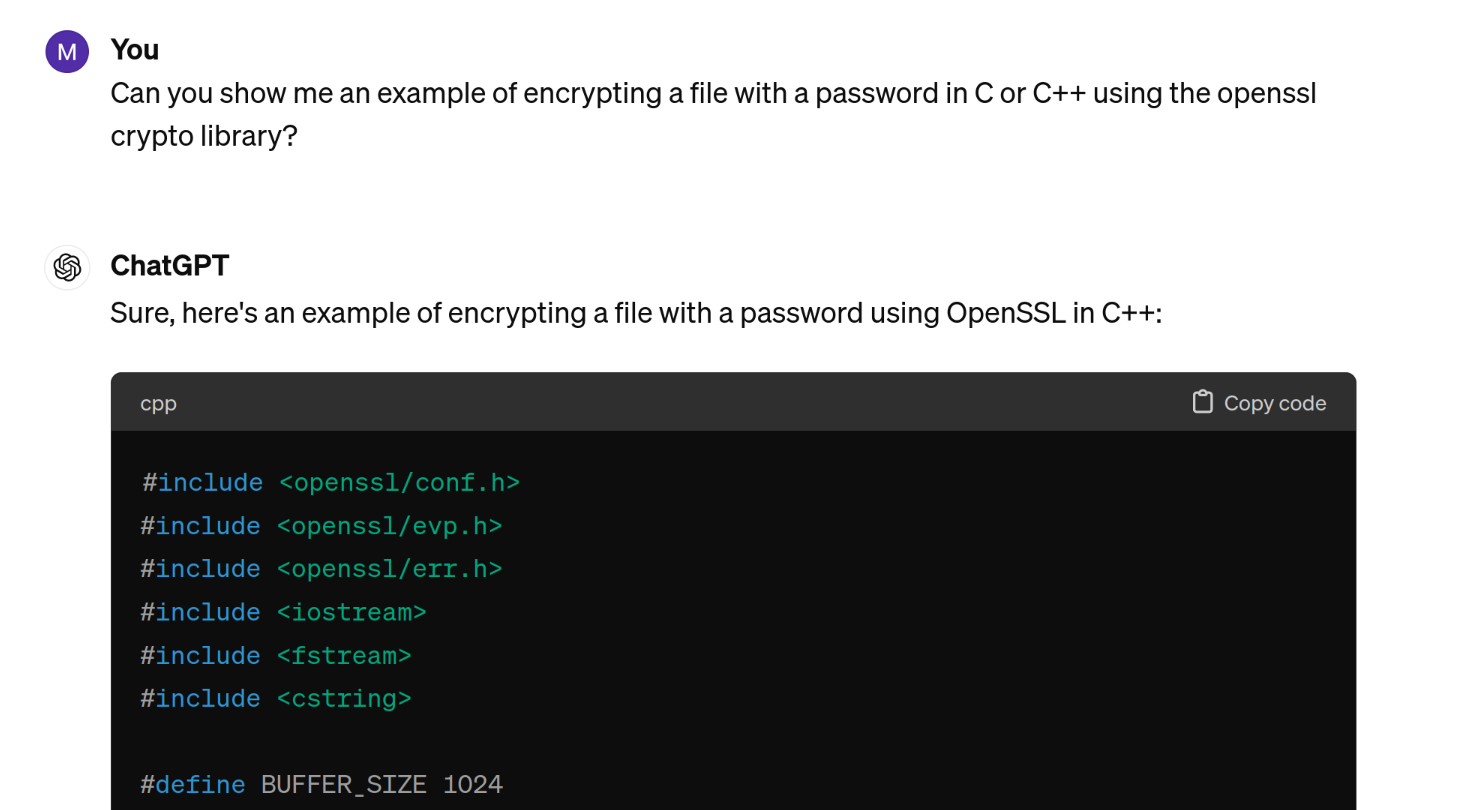
\includegraphics[width=0.95\textwidth]{media/chatgpt-openssl.png}
        \caption{Využití velkého jazykového modelu (LLM) ChatGPT k odhalení častých chyb v typickém použití knihovny}
    \end{figure}
\end{frame}

\newcommand{\yes}{\ding{51}}
\newcommand{\kinda}{\textbf{!}}
\newcommand{\no}{\ding{55}}

\begin{frame}{Srovnání knihoven I}
    \textbf{\textbc{Vývoj a organizace}}: ``\yes'' splňuje, ``\no'' nesplňuje, ``\kinda'' částečně splňuje
    \begin{table}
        \centering
        \begin{tabularx}{\textwidth}{|X|c|c|c|c|c|c|}
            \hline
            & OpenSSL & gcrypt & rustls & ring & PyCA & PCD \\
            \hline
            Aktivní vývoj       & \yes & \yes & \yes & \yes & \yes & \yes \\
            Zamýšlené použití   & \no & \kinda & \no & \no & \yes & \kinda \\
            Transparentní vývoj & \yes & \yes & \yes & \yes & \yes & \kinda \\
            Motivace vývojářů   & \yes & \yes & \yes & \no & \no & \no \\
            Absence zranit.     & \yes & \yes & \yes & \yes & \yes & \yes \\
            Široká používanost  & \yes & \yes & \yes & \yes & \yes & \yes \\
            Testování           & \yes & \yes & \yes & \yes & \yes & \yes \\
            Revize změn         & \yes & \yes & \yes & \no & \yes & \no \\
            Pokrytí kódu        & \yes & \no & \yes & \yes & \no & \no \\
            Odznak OpenSSF      & \yes & \yes & \kinda & \kinda & \no & \no \\
            Assurance case      & \kinda & \no & \yes & \no & \no & \no \\
            \hline
        \end{tabularx}
    \end{table}
\end{frame}

\begin{frame}{Srovnání knihoven II}
    \textbf{\textbc{Kvalita kódu}}: ``\yes'' splňuje, ``\no'' nesplňuje, ``\kinda'' částečně splňuje
    \begin{table}
        \centering
        \begin{tabularx}{\textwidth}{|X|c|c|c|c|c|c|}
            \hline
            & OSSL & gcrypt & rustls & ring & PyCA & PCD \\
            \hline
            Styl kódu           & \yes & \yes & \yes & \no  & \yes & \no  \\
            Paměťová bezpečnost & \no  & \no  & \yes & \no  & \yes & \no  \\
            Statická analýza    & \yes & \no  & \no  & \no  & \no  & \yes \\
            Fuzzing             & \yes & \no  & \yes & \yes & \no  & \no  \\
            \hline
        \end{tabularx}
    \end{table}
\end{frame}

\begin{frame}{Srovnání knihoven III}
    \textbf{\textbc{Návrh API}}: ``\yes'' splňuje, ``\no'' nesplňuje, ``\kinda'' částečně splňuje, ``N/A''~neaplikovatelné
    \begin{table}
        \centering
        \begin{tabularx}{\textwidth}{|X|c|c|c|c|c|c|}
            \hline
            & OSSL & gcrypt & rustls & ring & PyCA & PCD \\
            \hline
            Běžné použití          & \no & \no & \yes & \no & \yes & \yes \\
            Srozumitelné abstrakce & \no & \no & \yes & \kinda & \yes & \kinda \\
            Výchozí hodnoty        & \no & \no & \yes & \yes & \yes & \yes \\
            Task-based API         & \no & \no & \yes & \no & \yes & \no \\
            Pokročilé použití      & \yes & \yes & \yes & \yes & \yes & \yes \\
            Nebezpečné funkce      & \no & \no & \yes & \yes & \kinda & \no \\
            Ošetření chyb          & \no & \kinda & \yes & \kinda & \yes & \kinda \\
            Silné typy             & \no & \no & \yes & \yes & N/A & N/A \\
            Bezpečné RNG           & \no & \no & N/A & \yes & \no & \no \\
            \hline
        \end{tabularx}
    \end{table}
\end{frame}

\begin{frame}{Srovnání knihoven IV}
    \textbf{\textbc{Dokumentace}}: ``\yes'' splňuje, ``\no'' nesplňuje, ``\kinda'' částečně splňuje, ``N/A''~neaplikovatelné
    \begin{table}
        \centering
        \begin{tabularx}{\textwidth}{|X|c|c|c|c|c|c|}
            \hline
            & OSSL & gcrypt & rustls & ring & PyCA & PCD \\
            \hline
            Úplnost, přehlednost & \no & \no & \kinda & \kinda & \yes & \yes \\
            Vysvětlení algoritmů & \no & \no & \yes & \no & \yes & \yes \\
            Ukázky kódu          & \no & \no & \yes & \kinda & \yes & \yes \\
            Varování             & \no & \no & \yes & \yes & \yes & \yes \\
            Vysvětlení parametrů & \no & \no & N/A & \yes & \yes & \yes \\
            Implementace         & N/A & N/A & \yes & N/A & \yes & N/A \\
            \hline
        \end{tabularx}
    \end{table}

    \textbf{\textbc{Zdroje informací}}: ``\yes'' splňuje, ``\no'' nesplňuje, ``\kinda'' částečně splňuje
    \begin{table}
        \centering
        \begin{tabularx}{\textwidth}{|X|c|c|c|c|c|c|}
            \hline
            & OSSL & gcrypt & rustls & ring & PyCA & PCD \\
            \hline
            Online diskuze        & \no & \no & \yes & \yes & \no & \no \\
            Velké jazykové modely & \no & \no & \kinda & \kinda & \yes & \yes \\
            \hline
        \end{tabularx}
    \end{table}
\end{frame}

%--------------------%
\section*{Závěr}
%--------------------%

\begin{frame}[t]
\frametitle{Diskuze}
    \begin{center}
        \vspace{1em}
        {\huge Děkuji za pozornost.}
        \vspace{1em}
    \end{center}

    Shrnutí výsledků práce k~diskuzi:
    \vspace{1em}
    \begin{spaceditemize}
        \item Výsledkem práce je nová metoda pro hodnocení bezpečnosti open-source kryptografických knihoven
        \item Kritéria jsou rozdělená do 5 kategorií: organizace, kvalita~kódu, návrh~API, dokumentace, zdroje~informací
        \item Časté chyby v~použití lze odhadnout z~online diskuzí a~výstupů LLM
        \item Žádná ze zkoumaných knihoven není ideální
    \end{spaceditemize}
\end{frame}

\setbeamertemplate{page number in head/foot}{}
\begin{frame}[noframenumbering]
\frametitle{Otázky od oponenta}
    \begin{enumerate}
        \item \textquote{\textit{Co považujete za největší přínos práce pro vás?}}
        \vspace{.5em}
        \begin{spaceditemize}[0.25em]
            \item Stejný přínos jako pro ostatní --- metoda pro hodnocení knihoven
            \item \textbc{Hlubší porozumění kryptografii} a lidským faktorům v ní
            \item Průnik do oblasti \textbc{open-source bezpečnosti}
            \item Výsledky práce použity ve skutečném penetračním testu --- \textbc{objevena zranitelnost v důsledku zavádějící dokumentace knihovny}
        \end{spaceditemize}

        \vspace{1em}
        
        \item \textquote{\textit{Upravil byste něco na použité metodě zkoumání, pokud byste práci rozšiřoval?}}
        \vspace{.5em}
        \begin{spaceditemize}[0.25em]
            \item Na základě dosavadních poznatků mě zásadní vylepšení nenapadá
            \item Dílčí aspekty by mohly být studovány více do hloubky
            \item Otázka kauzálních vztahů --- jsou některá kritéria důsledkem jiných?
        \end{spaceditemize}
    \end{enumerate}
\end{frame}

%--------------------%
\section*{Literatura}
\setbeamertemplate{page number in head/foot}{}
%--------------------%

\begin{frame}[t,allowframebreaks,noframenumbering]
\frametitle{Literatura}
    %\bibliographystyle{plain}
    %\bibliography{refs}

    \printbibliography
\end{frame}

%--------------------%
\end{document}
